% !TEX program = arara
% arara: pdflatex
% arara: biber
% arara: pdflatex
% arara: pdflatex
\documentclass{pi1}
\begin{document}
% \maketitle	{Nummer}{Abgabedatum}{Tutor1-Name}{Tutor2-Name}{Gruppennummer}
%          		{Teilnehmer 1}{Teilnehmer 2}{Teilnehmer 3}
\maketitle{8}{16.12.2012}{Berghöfer/Senger}{8}
		{Beate Ruffer}{Mohamadreza Khostevan}{Leopold Schulz-Hanke}
% Beginn des eigentlichen Textes

\section{Alles super hier (20\%)}
In unserem Spiel sind 2 Klassen implementiert, deren Instanzen aufgehoben werden können: Hammer und Scissor. Sie besaßen schon seit einigen Abgaben die Superklasse \texttt{Collectable}. Auch die Klassen der Hindernisse Bush, Stone und Comb erbten schon von der Superklasse \texttt{Obstacle}. Da wir aber in vorherigen Aufgaben mit Hilfe vom \emph{instanceof}-Operator auf ein passendes Inventar prüfen sollten, war es nicht möglich das passende Inventar als Attribut zu hinterlegen und der Methode in der Superklasse die Prüfung zu überlassen. Nun haben wir ein Objektattribut \texttt{isBeatenBy} vom Typ Class eingeführt, mit dessen Hilfe der Vergleich durchgeführt wird. Somit können wir die prüfende Methode in die Superklasse Obstacle verschieben. Dadurch haben wir 3-Fach duplizierten Code in nur einer Methode zusammengeführt.

\begin{lstlisting}[caption={Klasse \emph{Obstacle}}, firstnumber=3, language=Java]
/**
 * Oberklasse für alle Hindernisse. Diese Klasse vereint alle Hindernisse,
 * so dass man leichter auf ein Hindernis prüfen kann.
 * 
 * @author Beate Ruffer (Bea), Mohamadreza Khostevan (Amir), Leopold Schulz-Hanke (Leo) 
 * @version 2.0.0
 * 
 */
public class Obstacle extends Actor
{   
    /**
     * Sound Datei, die abgespielt wird, wenn diese Hindernisse überwunden wurden.
     */
    public String beatenSound;
    
    /**
     * Definiert durch Objekte welcher Klasse das Hindernis überwunden werden kann
     */
    protected Class isBeatenBy;
    
    /**
     * Konstruktor von Obstacle wird von der Subklasse aufgerufen.
     * @param isBeatenBy Die Klasse des Objekts, welche das Hindernis überwinden kann.
     */
    public Obstacle(Class isBeatenBy){
        this.isBeatenBy = isBeatenBy;
    }
    
    /**
     * Prüft, ob das im Inventar enthaltene Objekt eine Instanz von isBeatenBy ist. Falls ja, wird das Hindernis von dem Objekt
     * im Inventar geschlagen und die Heldin kann passieren.
     * 
     * @param collectable Das zu prüfende Objekt.
     * @return true, wenn Hindernis überwunden ist.
     */
    public boolean isBeaten(Actor collectable)
    {
        return collectable.getClass() == isBeatenBy ;
    }
}

\end{lstlisting}

Nun müssen die Klassen der Hindernisse nur noch das passende Inventar (über den Konstruktor der Superklasse) und den Sound setzen.

\begin{lstlisting}[caption={Konstruktor von \emph{Stone}}, firstnumber=18, language=Java]
public Stone(){
        super(Hammer.class);
        beatenSound = "explosion.wav";
    }
\end{lstlisting}

\paragraph{Tests.}Da nun mal jedes kleine Refactoring Regression-Bugs hervorbringen kann, haben wir erneut getestet. Wir haben einen Hammer in unser Inventar aufgenommen, konnten wie erwartet keinen Bush oder Comb passieren. Nur der Stone konnte überwunden werden (der richtige Sound wurde auch abgespielt). Mit der Schere im Inventar konnten wir den Stone nicht überwinden, dafür aber Comb und Bush (ebenfalls mit den richtigen Sounds).

\section{Massenkarambolage (30\%)}
\label{s:collider}

\begin{enumerate}

\item
Methode
\begin{lstlisting}[caption={\emph{getCollidingObject(Class cls)}-Methode}, firstnumber=25, language=Java]
/**
     * Liefert das Objekt der Klasse cls mit dem eine Kollision besteht.
     * @param cls die Klasse, nach dessen Kollision geprüft wird
     * @return das Objekt, mit dem eine Kollision stattgefunden hat
     */
    public Actor getCollidingObject(Class cls){
        return getOneIntersectingObject(cls);
    }
\end{lstlisting}

\item
Methode
\begin{lstlisting}[caption={\emph{collidesWith(Class cls)}-Methode}, firstnumber=25, language=Java]
/**
     * Prüft, ob gerade eine Kollision besteht
     * @param cls die Klasse, auf deren Kollision geprüft wird
     * @return ob gerade eine Kollision mit einer Instanz der Klasse cls besteht
     */
    public boolean collidesWith(Class cls){
        return getCollidingObject(cls) != null;
    }
\end{lstlisting}

\item
Methode
\begin{lstlisting}[caption={\emph{newCollisionWith(Class cls)}-Methode}, firstnumber=25, language=Java]
/**
     * Prüft, ob gerade eine neue Kollision mit einer Instanz
     * der Klasse cls begonnen hat.
     * @param cls die Klasse, auf deren Kollision geprüft wird
     * @return ob gerade eine neue Kollision mit einer Instanz der Klasse cls begonnen hat
     */
    public boolean newCollisionWith(Class cls) {
        Crashable obj =  null;
        if ( collidesWith(cls) ){
            if (collisions.get(cls) == null || collisions.get(cls) != obj ){
                collisions.put(cls, obj);
                return true;
            }
        } 
        return false;
    }
\end{lstlisting}

\end{enumerate}

Erneut musste einiges an Refactoring gemacht werden. Alle Klassen, mit deren Instanzen die Biene  kollidieren kann, erben nun von \texttt{Crashable}. Jede Subklasse von Crashable hat nun auch eine Methode \texttt{handleCrash(Bee bee)} mit der sie auf (von der Biene registrierte) Kollisionen reagieren kann. Registriert die Biene eine Kollision, ruft sie den Crash Handler des Objektes auf, mit dem sie kollidiert. Dabei übergibt sie sich selbst als Paramter (für eventuelle Zugriffe auf das Inventar oder Scoreboard der Biene).

\section{Richtig kollidieren (50\%)}

Da nun alle Klassen, die mit der Biene kollidieren können, Subklassen von \texttt{Crashable} sind, braucht sie nicht mehr zu wissen mit welcher Subklasse von Crashable die Kollision stattfindet, sondern muss nur noch deren Crash Handler aufrufen.

\begin{lstlisting}[caption={\emph{checkCollisions()}-Methode}, firstnumber=156, language=Java]
/**
     * Prüft, ob die Biene mit einem Hindernis kollidiert. Falls eine Kollision stattfindet, wird
     * der Crash Handler des Objekts aufgerufen.
     */
    private void checkCollisions()
    {
        if (newCollisionWith(Crashable.class))  {
            Crashable crashable = (Crashable) getCollidingObject(Crashable.class);
            crashable.handleCrash(this);
        }
    }
\end{lstlisting}

Einzige Ausnahme dabei sind die \emph{Collectables}. Dies sind die Objekte, die in das Inventar aufgenommen werden können. Da nicht mit jedem act()-Aufruf auf Kollisionen mit Collectables geprüft werden soll, sondern nur auf Tastendruck, erben Collectables nicht von Crashable (und haben somit auch keinen Crash Handler). Es wird weiterhin auf Tastendruck die Methode takeOrFreeCollectable() aufgerufen. Diese nutzt aber zur Kollisionsprüfung nun unsere neuen Methoden.

\begin{lstlisting}[caption={\emph{takeOrFreeCollectable()}-Methode}, firstnumber=168, language=Java]
/**
     * Wenn ein Collectable in der Nähe und das Inventar leer ist, wird das Collectable eingesammelt.
     * Befindet sich ein Actor im Inventar, wird dieser an der aktuellen Position der Biene in die
     * Welt gesetzt. Andernfalls wird der Fehlerton abgespielt.
     */
    private void takeOrFreeCollectable()
    {
        if (newCollisionWith(Collectable.class) && myInventory.isEmpty() ){
            Collectable collectable = (Collectable) getCollidingObject(Collectable.class);
            myInventory.pushToInventory(collectable);
        } else if (!myInventory.isEmpty()){
            myInventory.removeFromInventory(this.getX(), this.getY());
        } else {
            Greenfoot.playSound("out.wav");
        }
    }
\end{lstlisting}

Kommen wir nun zur Implementierung der 3 Methoden zur Kollisionsprüfung.
Im Vergleich zu Aufgabe 2 haben wir nur die erste Methode erweitert.\\
\texttt{getCollidingObject(Class cls)} gibt uns das Objekt zurück, mit dem tatsächlich (also nicht nur die Bounding Box) eine Kollision stattfindet.

\begin{lstlisting}[caption={\emph{getCollidingObject(Class cls)}-Methode}, firstnumber=22, language=Java]
/**
     * Liefert das Objekt der Klasse cls, mit dem eine Kollision besteht.
     * @param cls die Klasse, nach dessen Kollision geprüft wird
     * @return das Objekt, mit dem eine Kollision stattgefunden hat
     */
     public Actor getCollidingObject(Class cls){
        List<Actor> objects = getIntersectingObjects(cls);
        
        for (Actor object : objects){
                for (int x = 0; x < this.getImage().getWidth(); x++){
                    for (int y = 0; y < this.getImage().getHeight(); y++){
                        if (this.getImage().getColorAt(x, y).getAlpha() > 0){
                            double rotation = Math.toRadians(this.getRotation());
                            double dx = x - this.getImage().getWidth() / 2;
                            double dy = y - this.getImage().getHeight() / 2;
                            int xWorld = (int) (this.getX() + dx * Math.cos(rotation) - dy * Math.sin(rotation));
                            int yWorld = (int) (this.getY() + dx * Math.sin(rotation) + dy * Math.cos(rotation));
                            if (pixelsWithinImageBounds(object, xWorld, yWorld) && visiblePixelAt(xWorld, yWorld, object)){
                                if (testMode){
                                    this.getImage().setColorAt(x, y, Color.RED);
                                } else {
                                    return object;
                                }
                            }                            
                        }
                    }
                }
            
        }
        return null;
    }
\end{lstlisting}

Zunächst speichern wir eine Liste mit allen kollidierten Objekten (noch Bounding Box). Diese Liste wird durchlaufen und darin wird jeweils jedes Pixel des Bildes durchlaufen (Zeilen 31 \& 32).\\
Im Falle eines nicht-transparenten Pixels (Zeile 33) wird dieses Pixel in die Weltkoordinaten umgerechnet. Anhand dieser Koordinaten können wir dann die Koordinaten im kollidierenden Objekt errechnen. Doch vorher müssen wir prüfen, ob diese Koordinaten überhaupt innerhalb des kollidierten Objekts liegen. Dies geschieht mit \texttt{pixelsWithinImageBounds(Actor obj, int x, int y)}.

\begin{lstlisting}[caption={\emph{pixelsWithinImageBounds(Actor obj, int x, int y)}-Methode}, firstnumber=97, language=Java]
/**
     * Prüft, ob ein die Koordinaten innerhalb des Bildes eines Objektes liegen
     * @param obj Das zu Prüfende Objekt
     * @param x X-Koordinate
     * @param y Y-Koordinate
     * @return true, wenn die Koordinaten innerhalb des Bildes liegen
     */
    private boolean pixelsWithinImageBounds(Actor obj, int x, int y){
        int xStart = obj.getX() - obj.getImage().getWidth() / 2;
        int xEnd = xStart + obj.getImage().getWidth();
        int yStart = obj.getY() - obj.getImage().getHeight() / 2;
        int yEnd = yStart + obj.getImage().getHeight();
        return x >= xStart && x < xEnd && y >= yStart && y < yEnd;
    }
\end{lstlisting}

Liegen die Koordinaten also innerhalb des kollidierenden Objekts, können die Weltkoordinaten in die Bildkoordinaten dieses Objekts umgerechnet werden. Dann wird geprüft, ob auch dieses Pixel nicht-transparent ist.

\begin{lstlisting}[caption={\emph{visiblePixelAt(int xWorld, int yWorld, Actor obj)}-Methode}, firstnumber=80, language=Java]
/**
     * Rechnet Weltkoordinaten in die Bildkoordinaten des Actors um und prüft
     * ob dort ein sichtbarer Pixel ist
     * @param xWorld x-Weltkoordiante
     * @param yWorld y-Weltkoordinate
     * @param obj Das Objekt, in dessen Bildkoordinaten umgerechnet werden soll
     * @return true, wenn an den Koordinaten ein sichtbarer Pixel ist
     */
    private boolean visiblePixelAt(int xWorld, int yWorld, Actor obj){
        double rotation = Math.toRadians(obj.getRotation());
        int dx = xWorld - obj.getX();
        int dy = yWorld - obj.getY();
        int xInObject = (int) (obj.getImage().getWidth() / 2 + dx * Math.cos(rotation) + dy * Math.sin(rotation));    
        int yInObject = (int) (obj.getImage().getHeight() / 2 - dx * Math.sin(rotation) + dy * Math.cos(rotation));
        return (obj.getImage().getColorAt(xInObject, yInObject).getAlpha() > 0 );
    }
\end{lstlisting}

Liefern pixelsWithinImageBounds() und visiblePixelAt() beide true zurück, wird das Objekt, mit dem dann tatsächlich eine Kollision stattgefunden hat, zurückgeliefert. Dies geschieht aber nicht im testMode. In dem Fall wird lediglich das entsprechende Pixel rot gefärbt (Listing 8 Zeile 40).\\
Der testMode ist ein Objektattribut in Collider. Dieser kann auf Wunsch einfach auf true gesetzt werden.

\paragraph{Tests.}
Die Superklasse Collider  sowie ihre Methoden und Teilabschnitte mussten anfangs durch kleinere Testausgaben überprüft werden. Zu diesen Tests zählten beispielsweise die Systemausgaben und die Verwendung des integrierten TestModus.

Um zu garantieren, dass die Collider Superklasse und ihre Kollisionserfassung nicht nur theoretisch funktionieren, wurde es notwendig diese Methode und ihre Modifikationen in die Grundfunktionen des Spielers und anderer kollisionsabhängiger Klassen zu integrieren. Vorläufig wurde hierfür die Bee Klasse modifiziert um die Methoden der Superklasse an der Positionswiederherstellung zu prüfen.

Bei eingeschaltetem Testmodus werden alle Pixel gefärbt, bei denen eine Kollision registriert wird.
Es ist hieran einfach das Auslösen des Kollisionstests zu demonstrieren.

Nach dem Erstellen einer funktionstüchtigen Methode bestanden die Tests nicht mehr hauptsächlich in einem Funktionsnachweis, sondern in der Kopplung mit anderen Klassen. So musste zum Beispiel die Positionswiederherstellung sowie die Erfassung von Items, Hindernissen und aufsammelbaren Objekten an die neue Methode angeknüpft werden.
Um eine "globale" Kollisionserfassung für die existierenden Klassen zu ermöglichen, mussten zumal viele von diesen in ihrem Aufbau verändert werden.

Die unten gezeigten Bilder demonstrieren beispielhaft einige Tests, die wir unter Verwendung des TestModus der Collider-Klasse durchgeführt haben.

\begin{figure}[h]
	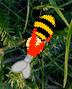
\includegraphics[scale=1]{testMode1.png}
	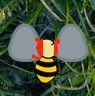
\includegraphics[scale=1]{testMode2.png}
	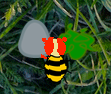
\includegraphics[scale=1]{testMode3.png}
	\caption{Kollision mit Unterklassen vonObstacle und Collectable}
	\label{bild1}
\end{figure}



Hierzu zählen gleichzeitige Kollisionen mit mehreren Objekten einer Klasse, gleichzeitige Kollisionen mit mehreren Objekten verschiedener Klassen und mit jenen Objekten einer unabhängigen Superklasse.
Es wird durch die Färbung deutlich, dass all diese Kollisionen registriert werden.


Die genannten Beispiele sind wichtig in Anbetracht der Rolle, welche die Superklasse Collider ab jetzt übernehmen soll, nämlich jene über die Klasse Bee eine Erfassung und Interaktion mit allen Objekten zu ermöglichen.\newline

Zu den oben gezeigten Tests kommt also hinzu, dass die Kollision nicht nur erkannt werden müssen, sondern auch erfolgreich zwischen den Objekten differenzieren können müssen um deren notwendige Funktionen auszulösen.
Somit sollen ab jetzt Unterklassen von Collectable mit dieser Methode aufgenommen werden können und Kollisionen über die Methoden von Collider zum Aufhalten der Biene führen.
Die besagte Zweckmäßigkeit der Klassen und ihrer Objekte wurde von uns natürlich ebenfalls überprüft.

\end{document}

